\vspace{5cm}
\subsection{El Concepte de 3BLD}

Per començar cal entendre el funcionament d'una resolució de blind, primer el cub és barrejat per una persona i el posa dins d'una capsa o un cube cover\footnote{Un cube cover és una tapa per cubs feta de cartró i que s'utlitza a les competicions}, després es col·loca a la taula boca avall i la persona que l'ha de resoldre es pren el seu temps per respirar. 
Un cop fet això la persona que resol el cub encén el timer i destapa el cub, de manera que el temps comença a comptar i es comença a memoritzar. Un cop acabada la memorització el que resol el cub es tapa els ulls amb un antifaç i comença a resoldre el cub, mentre que una persona externa li posa una cartiluna entre el cub i la seva cara per evitar trampes i mirar per sota de l'antifaç.
Tots aquests passos s'han d'executar perfectament perr asegurar-se de la resolució compti.

\begin{figure}[ht]
    \centering
    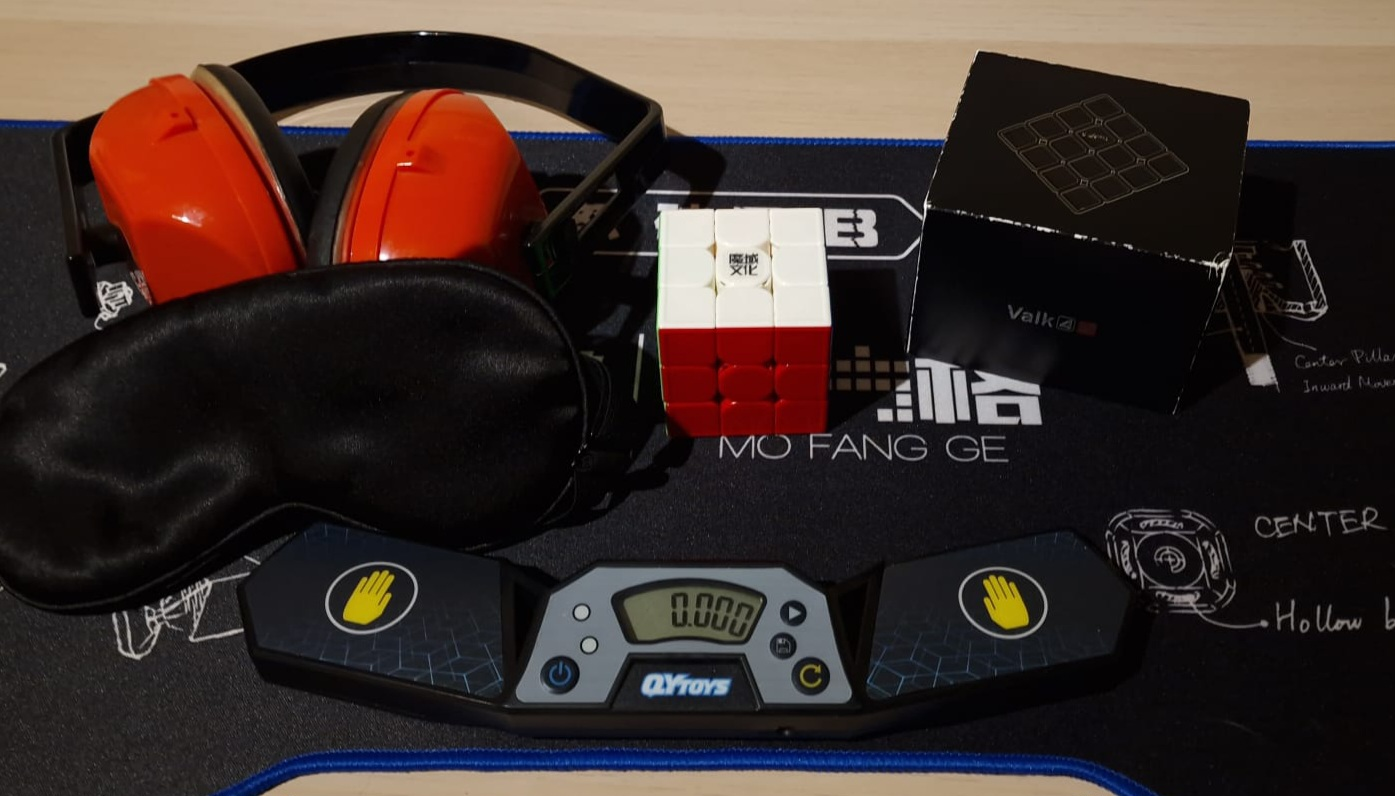
\includegraphics[width=12cm]{img/figures/materials-bld.jpg}
\caption{Materials necessaris per poder executar blind}
    \label{fig:materials-bld}
\end{figure}

En la imatge anteriori es poden veure el timer\footnote{El timer és el compatdor amb la forma de les mans que es veu al centre de la imatge}, l'antifaç, la caixa per cobrir el cub, que en aquest cas jo utlizo una que tinc d'un cub, i a més a més uns cascos d'obra per aïllarte del soroll ambient.

\vspace{0.5cm}
\subsection{Fases de la Resolució}

Com ja he esmentat a la seccio anterior, completar el cub de Rubik amb els ulls tancats, es divideix en dos grans fases, memorització i execució. I dins d'aquestes fases hi han diferents procediments per poder aconseguir fer-ho correctament.

\subsubsection{Memorització}

Durant aquesta fase de memorització, com ja ho diu el seu nom, s'ha de memoritzar el cub. Molta gent pensa que els speedcubers que practiquem blind memoritzem el cub color per color mitjançant la memòria fotogràfica, però la veritat no és així, perquè la memòria fotogràfica només la té molt poca gent, i bé, jo m'enrecordo dels objectes que tinc a la taula si tanco els ulls ara mateix, però memoritzar el cub d'aquesta manera porta molt de temps i no és la més eficient de fer-ho.
El que fem es convertir aquestes posicions on estan les peçes del cub, que "només" són 20 en lletres i ho fem d'una manera distribuida en ordre que nosaltres ens memoritzem. L'esquema de lletres\footnote{És la distribució de lletres} que utilizo és el que es veu a la següent figura.

\begin{figure}[ht]
    \centering
    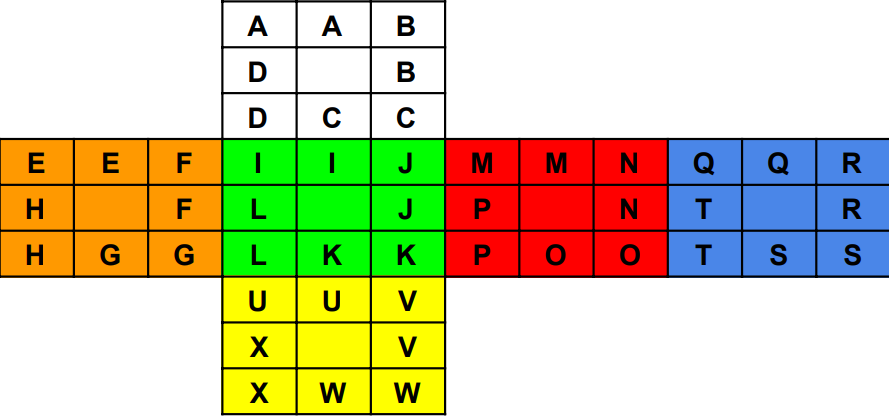
\includegraphics[width=12cm]{img/figures/letter-scheme.png}
\caption{Esquema de LLetres}
    \label{fig:letter-scheme}
\end{figure}

Com es pot veure hi han lletres repetides i això és degut a que hi ha memorització per arestes i memorització per cantonades. Com està mencionat a la secció 1.2.2 en el cub hi ha 8 arestes i 12 cantonades, per tant haig de memoritzar respectivament 12 lletres d'arestes i 8 lletres de cantonades.
Un altre cop tenim el problema de que no és gaire eficient memoritar les lletres una per una i és per això que la manera correcta de fer-ho és:
\\\\Memoritzar dos lletres i amb aquestes dos lletres formar una paraula de la qual puguis pensar en una imatge en la que et puguis enrecordar. En resum, és converir parells de lletres en en imatges, per tant ara tenim la meitat d'ítems a memoritzar. Un exemple d'aquesta fusío de lletres és. 
\vspace{0.25cm}

$$ \textrm{Haig de memoritzar les lletres R i B    }  \rightarrow \textrm{   RedBull} $$
$$ \textrm{Haig de memoritzar les lletres A i C   }  \rightarrow \textrm{   Aire Acondicionat (AC és el símbol)} $$

\vspace{0.33cm}

De maner pràctica es comença a memortizar desde la peça UK mirant el color de U, de la lletra en la posicó U que és la inicial i treus una lletra i llavors mires a la posció on hi ha d'anar aquesta primera lletra que has trobat i mires quina lletra treus, i així fins que memoritzis totes les arestes i després fas el mateix amb les cantonades. És una concepte díficl d'explicar amb paraules i es veu millor al següent exemple. Cal destacar que al començar a memortizar la posció UK la saps perquè poses el centre verd mirant cap a tu i el centre blanc mirant cap a dalt.
\\\\BARREJA: F2 B R2 U'L2 U2 B' L' F2 U' B2 U L2 U R2 F2 L2 U' L2 F

\begin{figure}[h!]
    \centering\RubikCubeSolvedWY
    \RubikRotation{Y,F2,B,R2,Up,L2,U2,Bp,Lp,F2,Up,B2,U,L2,U,R2,F2,L2,Up,L2,F}
    \ShowCube{8cm}{0.6}{\DrawRubikCubeF}
    \caption{Cub barrejat per exemple de Blind}
    \label{exemple-memo}
    \end{figure}

Començem mirant all lloc de U K com a l'esquema de lletres i veiem que és blanca a lloc U i taronja al lloc K, llavors ens fixem mirem l'esquema de lletres en l'aresta blanca-taronja i veiem que és la lletra D. 
Després ens fixem en el lloc de la lletra D i està una peça blanca-verda que és la lletra C, però és un cas especial, que més tard parlo a la secció d'execució però aquesta C es converteix en W, no s'ha de saber res més, només és per tenir el concepte entès. Això ho fem succesivament i obtenim que les lletres totals que ens hem de memoritzar són:

$$ \textrm{Memorització Arestes: DW LA BV PX RI GT N } $$ $$ \textrm{(En aquest cas surten 13 perquè ha sigut una barreja amb cas especial)} $$
\vspace{0.33cm}
$$ \textrm{Memorització Cantonades: U MH VS MC} $$ $$ \textrm{(Igual que amb les arestes al ser un cas especial el valor es veu afectat)} $$
\vspace{0.33cm}
$$ \textrm{Memorització Total DW LA BV PX RI GT NU MH VS MC } $$

\begin{table}[h!]
    \begin{tabular}{|c|c|}
        \hline
    DW &             \\\hline
    LA & Los Ángeles \\\hline
    BV &             \\\hline
    PX &              
    \end{tabular}
    \end{table}

 
        
    






